\documentclass[tikz,border=8pt]{standalone}
\usepackage{amsmath,amssymb}
\usetikzlibrary{arrows.meta,automata,positioning,quotes}
\begin{document}
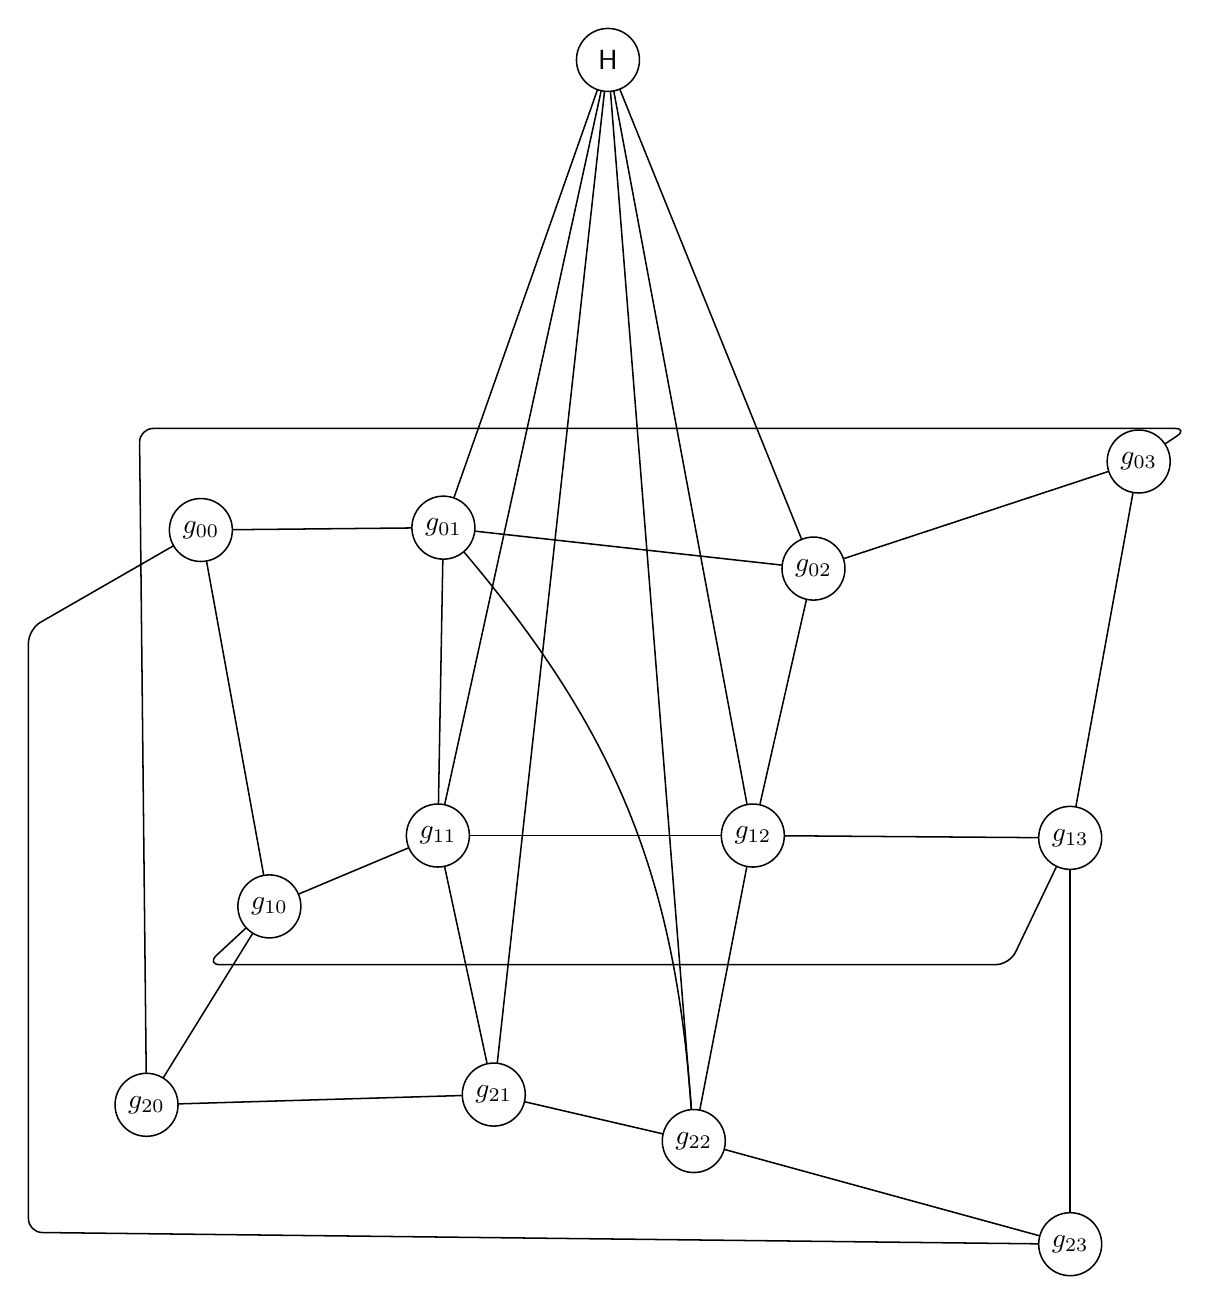
\begin{tikzpicture}[x=1cm,y=1cm]
\tikzset{
  graphnode/.style={circle,draw=black,line width=0.55pt,minimum size=8mm,inner sep=1pt,font=\sffamily},
  graphedge/.style={draw=black,line width=0.55pt,line cap=round,line join=round},
  directed/.style={graphedge,-{Stealth[length=2.4mm,width=2.0mm]}},
  undirected/.style={graphedge}
}
\node[graphnode] (n_g00) at (-0.70,0.74) {$g_{00}$};
\node[graphnode] (n_g01) at (2.38,0.77) {$g_{01}$};
\node[graphnode] (n_g02) at (7.08,0.25) {$g_{02}$};
\node[graphnode] (n_g03) at (11.21,1.61) {$g_{03}$};
\node[graphnode] (n_g10) at (0.17,-4.04) {$g_{10}$};
\node[graphnode] (n_g11) at (2.31,-3.14) {$g_{11}$};
\node[graphnode] (n_g12) at (6.31,-3.14) {$g_{12}$};
\node[graphnode] (n_g13) at (10.34,-3.17) {$g_{13}$};
\node[graphnode] (n_g20) at (-1.39,-6.56) {$g_{20}$};
\node[graphnode] (n_g21) at (3.02,-6.43) {$g_{21}$};
\node[graphnode] (n_g22) at (5.56,-7.02) {$g_{22}$};
\node[graphnode] (n_g23) at (10.34,-8.33) {$g_{23}$};
\node[graphnode] (n_H) at (4.47,6.71) {H};
\draw[undirected] (n_g00) -- (n_g01);
\draw[undirected] (n_g01) -- (n_g02);
\draw[undirected] (n_g02) -- (n_g03);
\draw[undirected] (n_g10) -- (n_g11);
\draw[undirected] (n_g11) -- (n_g12);
\draw[undirected] (n_g12) -- (n_g13);
\draw[undirected] (n_g20) -- (n_g21);
\draw[undirected] (n_g21) -- (n_g22);
\draw[undirected] (n_g22) -- (n_g23);
\draw[undirected] (n_g00) -- (n_g10);
\draw[undirected] (n_g10) -- (n_g20);
\draw[undirected] (n_g01) -- (n_g11);
\draw[undirected] (n_g11) -- (n_g21);
\draw[undirected] (n_g02) -- (n_g12);
\draw[undirected] (n_g12) -- (n_g22);
\draw[undirected] (n_g03) -- (n_g13);
\draw[undirected] (n_g13) -- (n_g23);
\draw[undirected] (n_H) -- (n_g01);
\draw[undirected] (n_H) -- (n_g02);
\draw[undirected] (n_H) -- (n_g11);
\draw[undirected] (n_H) -- (n_g12);
\draw[undirected] (n_H) -- (n_g21);
\draw[undirected] (n_H) -- (n_g22);
\draw[undirected,rounded corners=5pt] (n_g00) -- (-2.89,-0.52) -- (-2.89,-8.18) -- (n_g23);
\draw[undirected,rounded corners=5pt] (n_g03) -- (11.84,2.03) -- (-1.48,2.03) -- (n_g20);
\draw[undirected,rounded corners=5pt] (n_g10) -- (-0.63,-4.78) -- (9.57,-4.78) -- (n_g13);
\draw[undirected] (n_g01) to[bend left=18] (n_g22);
\end{tikzpicture}
\end{document}
